\chapter{Staggered Grids}
\label{chpt:staggered}

In Chapter~\ref{chpt:FDM} every problem had a single unknown $\phi$ and we were free to choose the grid it lived on. Many PDEs of interest instead couple \emph{several} unknowns together, such as the velocity and pressure of a fluid. This chapter introduces staggered grids, which place each unknown on its own grid. The choice matters: a placement of pressure on a grid that seems natural can produce a linear system with spurious, non-physical solutions! We will see that a staggered grid is nothing more than the Type~I and Type~II grids of Sections~\ref{sec:typeI} and~\ref{sec:typeII} used in combination, so the boundary condition tools from Chapter~\ref{chpt:FDM} and \ref{sec:bvp-example} carry over directly. We close the chapter by setting up a two-dimensional flow problem on a staggered grid.
\index{staggered grid}

\section{Coupled Unknowns on a Single Grid}
\label{sec:collocated}

Consider a one-dimensional problem with unknowns velocity $u(x)$ and pressure $p(x)$ on the periodic domain $[a,b]$. Suppose we place \emph{both} unknowns on the same Type~I grid $\{x_i\}$ (collocated grid layout) and approximate the pressure gradient with the second-order central difference~\eqref{eq:fdCentral}:
\index{collocated grid}
\begin{equation}
    p'_P \approx \frac{p_E - p_W}{2\,\Delta x}.
    \label{eq:stg-colGrad}
\end{equation}
Notice that $p_P$ itself never appears in~\eqref{eq:stg-colGrad}! The gradient at even-indexed points depends only on odd-indexed pressures, and vice versa. The pressure is effectively split across two independent sub-grids that never communicate---this is known as the checkerboard problem. Because the two sub-grids are decoupled, a "constant" pressure that alternates in sign from point to point has a discrete gradient of zero. Such a mode lies in the null space of the linear system so it can be added to any computed pressure without changing anything else. Therefore, computed pressures often show non-physical oscillations that resemble a checkerboard!
\index{checkerboard problem}

One could avoid the checkerboard issue by using one-sided differences, but as discussed in Chapter~\ref{chpt:FDM}, these are only first-order accurate. We would like a difference that is \emph{compact} (it uses neighboring values), centered, and second-order accurate.

\section{Staggering in One Dimension}
\label{sec:stg1D}

Recall from Section~\ref{sec:typeII} that a difference across two neighboring points (i.e., $P$ and $E$, or $W$ and $P$) is naturally centered and second-order accurate at the point halfway between them. On a \textbf{staggered grid}, different unknowns live at different, offset locations, and derivative calculations take advantage of this naturally second-order difference between two neighbors. In one dimension we partition $[a,b]$ into $N$ cells of width $\Delta x$ and place
\begin{itemize}
    \item the pressure $p$ at the cell centers $x_{i+1/2}$, labelled with stars (a Type~II grid), and
    \item the velocity $u$ at the cell faces $x_i$, labelled with circles (a Type~I grid).
\end{itemize}
This layout is shown in Figure~\ref{fig:stg-1D}. We extend the compass notation of Chapter~\ref{chpt:FDM}: for a cell centered at $P$, the neighboring cell centers are still $W$ and $E$, while the faces of cell $P$ are denoted by lowercase letters $w$ and $e$. Using neighbors to compute derivatives produces the pressure derivative at the faces (where the velocity $u$ is defined) and the velocity derivative at the centers (where the pressure is defined), so
\begin{align}
    p'_e &\approx \frac{p_E - p_P}{\Delta x}, \label{eq:stg-grad1D}\\[1mm]
    u'_P &\approx \frac{u_e - u_w}{\Delta x}. \label{eq:stg-div1D}
\end{align}
Each of these is a difference between immediate neighbors, centered exactly on the point where it is needed. Because every pressure value now appears in the derivative at the faces on either side of it, the sub-grids are coupled and the checkerboard problem is removed.

\begin{figure}[htbp]
    \centering
\includegraphics[page=2, width=\linewidth]{StaggeredGrids/images/staggeredMain.pdf}
    \caption{A one-dimensional staggered grid. Pressure $p$ lives at cell centers (Type~II, stars) and velocity $u$ lives at cell faces (Type~I, circles). Cell centers are labelled with uppercase compass letters and faces with lowercase letters.}
    \label{fig:stg-1D}
\end{figure}

On a domain with $N$ cells there are $N$ cell centers (where pressure lives) and $N + 1$ faces (where $u$ lives). On a periodic domain the first and last faces are the same physical point, leaving $N$ distinct faces. Writing~\eqref{eq:stg-grad1D} for every face defines a gradient operator $G$ that maps cell values to face values, and writing~\eqref{eq:stg-div1D} for every cell defines a divergence operator $D$ that maps face values to cell values.
\index{staggered grid!gradient operator}\index{staggered grid!divergence operator}

\begin{exercise}
For a periodic domain with $N$ cells:
\begin{enumerate}[label=(\alph*)]
    \item Write out $G$ and $D$ for $N=5$. Be careful about which face is indexed alongside which cell.
    \item Show that $D = -G^T$. What property of the continuous operators does this mimic? \emph{Hint: integrate $u\,p'$ by parts on a periodic domain.}
\end{enumerate}
\end{exercise}

\begin{remark}
Staggering is not free. Since $u$ and $p$ no longer share locations, any quantity that combines them, or any plot of them together, requires \textbf{interpolation} between grids, which is discussed further in Section~\ref{sec:stg-post}.
\end{remark}

\section{The Marker-and-Cell Grid}
\label{sec:mac}

The two-dimensional staggered grid most commonly used is the \textbf{Marker-and-Cell} (MAC) grid. Consider the domain $[a,b]\times[c,d]$ partitioned into $N_x \times N_y$ rectangular cells with
\index{MAC grid}\index{staggered grid!MAC}
$$
\Delta x = \frac{b-a}{N_x}, \qquad \Delta y = \frac{d-c}{N_y}, \qquad x_i = a + i\,\Delta x, \qquad y_j = c + j\,\Delta y.
$$
The velocity $\mathbf{u} = [u(x,y), v(x,y)]$ has two components and each is given its own grid, where
\begin{itemize}
    \item the horizontal component $u_{i,\,j+1/2}$ lives on the east and west faces $(x_i,\,y_{j+1/2})$ (squares), and
    \item the vertical component $v_{i+1/2,\,j}$ lives on the north and south faces $(x_{i+1/2},\,y_j)$ (triangles).
\end{itemize}
We also define the pressure $p(x,y)$, which lives at the cell centers $(x_{i+1/2},\,y_{j+1/2})$ (circles). The compass notation extends to two dimensions with $N$ and $S$ for the neighboring cell centers, and $n$ and $s$ for the faces of cell $P$, where east is the direction of increasing $x$ and north is the direction of decreasing $y$. Table~\ref{tab:stg-mac} summarizes the placement in terms of the grid types of Chapter~\ref{chpt:FDM}, and Figure~\ref{fig:stg-macCell} depicts the grid with a stencil for one cell.

\begin{table}[h!]
    \centering
    \begin{tabular}{|>{\raggedright\arraybackslash}p{2.3cm}|>{\raggedright\arraybackslash}p{3.3cm}||>{\raggedright\arraybackslash}p{2.6cm}|>{\raggedright\arraybackslash}p{2.6cm}|}
        \hline
        \textit{Unknown} & \textit{Location} & \textit{Grid in $x$} & \textit{Grid in $y$} \\
        \hline
        $p$ & cell centers & Type II & Type II \\
        $u$ & east/west faces & Type I & Type II \\
        $v$ & north/south faces & Type II & Type I \\
        \hline
    \end{tabular}
    \caption{Placement of unknowns on the MAC grid, described by the grid type each unknown sees in each coordinate direction.}
    \label{tab:stg-mac}
\end{table}

\begin{figure}[htbp]
    \centering
    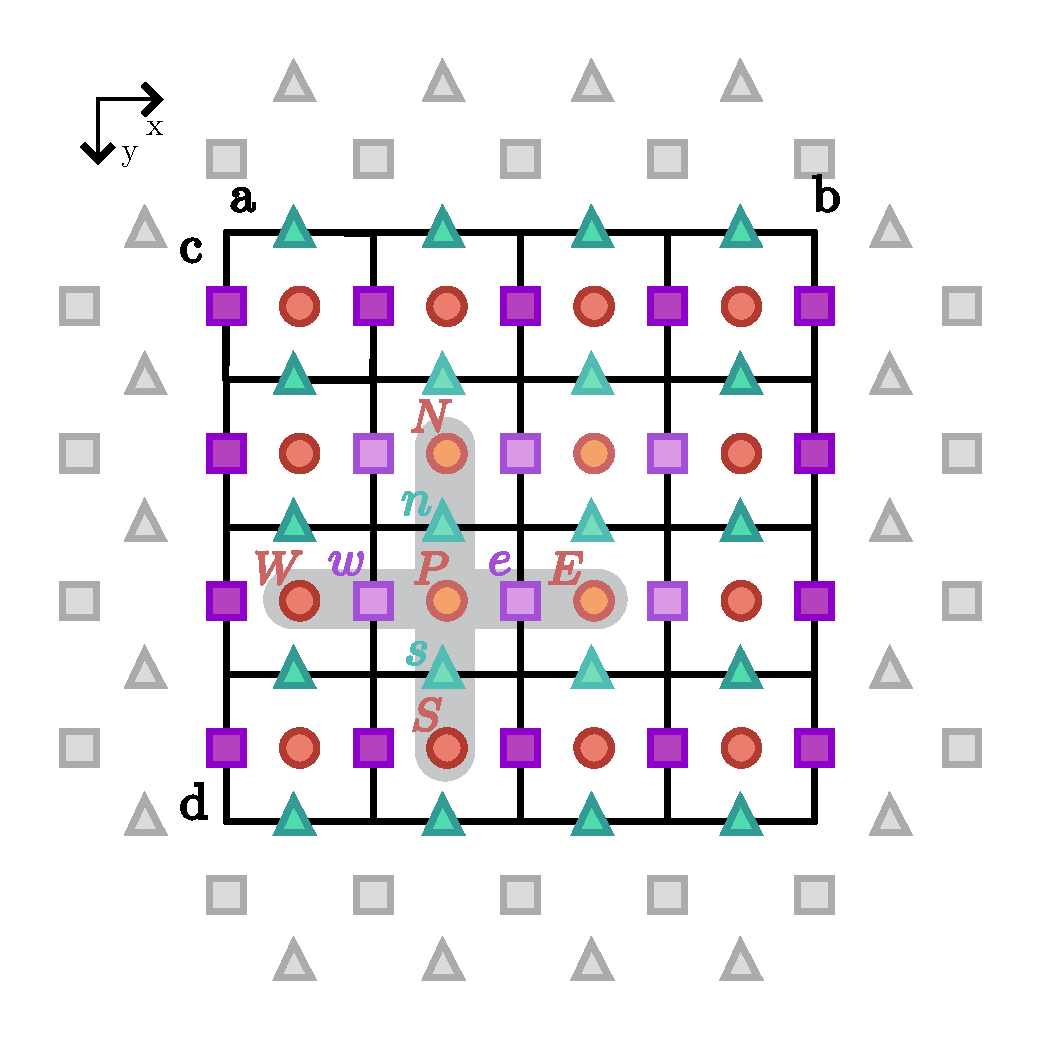
\includegraphics[page=1, width=\linewidth]{StaggeredGrids/images/staggeredMain.pdf}
    \caption{Depiction of MAC staggered grid in two-dimensions for $N_x = N_y = 4$. Pressure lives at the cell center (circles), horizontal velocity $u$ on the east and west faces (squares), and vertical velocity $v$ on the north and south faces (triangles). Ghost cells are shown for the velocity components only.}
    \label{fig:stg-macCell}
\end{figure}

\clearpage

Note that each component lives on the faces it carries fluid \emph{through}: $u$ measures flow across east and west faces, $v$ across north and south faces. The divergence evaluated at the cell center,
\begin{equation}
    (\nabla\cdot\mathbf{u})_P \approx \frac{u_e - u_w}{\Delta x} + \frac{v_s - v_n}{\Delta y},
    \label{eq:stg-div2D}
\end{equation}
is then the net flow out of cell $P$ per unit area. The discrete statement $\nabla\cdot\mathbf{u}=0$ becomes an exact balance of what flows into and out of each cell, which is a strong physical reason to prefer this layout.

\begin{exercise}
Write the MAC approximations of $\partial p/\partial x$ at the location of $u_e$ and of $\partial p/\partial y$ at the location of $v_n$ in compass notation.
\end{exercise}

Because each unknown lives on its own grid, each has its own set of ghost points, and boundary conditions must be imposed separately for each grid, which we discuss in the following sections.


\subsection{Ordering Unknowns}
\label{sec:stg-order}

In two dimensions the unknowns form a 2D array, but a linear system needs a single vector. We must choose an ordering that maps each pair $(i,j)$ to a single index $k$. In this text we will use row-wise stacking with the $x$-index varying fastest:
\begin{equation}
    k = i + j\,n_x, \qquad i = 0,\dots,n_x-1, \qquad j = 0,\dots,n_y-1,
    \label{eq:stg-order}
\end{equation}
where $n_x$ and $n_y$ are the number of unknowns of that variable in each direction and $j=0$ is the row nearest $y=c$. Note that $n_x$ and $n_y$ depend on the boundary conditions, as discussed in Section~\ref{sec:stokes}. We end with a vector of the form
\begin{equation}
\begin{bmatrix}
\mathbf{u} & \mathbf{v} & \mathbf{p}
\end{bmatrix}^T, \label{eq:unknowns}
\end{equation}
where $u(x,y)$, $v(x,y)$, and $p(x,y)$ have been flattened to the vectors $\mathbf{u}$, $\mathbf{v}$, and $\mathbf{p}$, respectively.


\subsection{Building Two-Dimensional Operators}
\label{sec:stg-kron}
\index{Kronecker product}

Recall that two-dimensional operators can be assembled either entry-by-entry or with the Kronecker product---both of these methods were discussed in Section~\ref{sec:bvp-example}. Whichever method you choose, \emph{look at your matrices}! A sparsity plot (\lstinline|plt.spy| in python, \lstinline|spy| in MATLAB) shows the nonzero entries of a matrix and reveals misplaced periodic entries, missing diagonals, and wrong block sizes. It is a great debugging tool!


\section{The Stokes Equations}
\label{sec:stokes}

When a fluid moves slowly enough, or is viscous enough, its inertia is negligible and its motion is governed by the \textbf{Stokes} equations:
\begin{align}
    \mu\,\nabla^2\mathbf{u} - \nabla p &= \mathbf{0}, \label{eq:stg-stokesMom}\\
    \nabla\cdot\mathbf{u} &= 0. \label{eq:stg-stokesCont}
\end{align}
On a domain $(x,y)\in\Omega = [0,1]\times[0,1]$, $\mathbf{u} = [u(x,y),\,v(x,y)]$ is the fluid velocity, $p(x,y)$ is the pressure, and $\mu>0$ is the viscosity. Equation~\eqref{eq:stg-stokesMom} is a balance between viscous forces and pressure forces, and~\eqref{eq:stg-stokesCont} states that the fluid is incompressible. The Stokes equations can model the swimming of bacteria and other microorganisms, the settling of fine particles, and the slow flow of very viscous fluids such as magma, glass, and polymer melts. Written out in components, the equations are
\begin{align}
    \mu\left(\frac{\partial^2 u}{\partial x^2} + \frac{\partial^2 u}{\partial y^2}\right) - \frac{\partial p}{\partial x} &= 0, \label{eq:stg-xmom}\\
    \mu\left(\frac{\partial^2 v}{\partial x^2} + \frac{\partial^2 v}{\partial y^2}\right) - \frac{\partial p}{\partial y} &= 0, \label{eq:stg-ymom}\\
    \frac{\partial u}{\partial x} + \frac{\partial v}{\partial y} &= 0. \label{eq:stg-cont}
\end{align}

Notice that~\eqref{eq:stg-stokesMom}--\eqref{eq:stg-stokesCont} contain no equation for the pressure on its own. The pressure appears only through $\nabla p$ and takes whatever values are needed to make the velocity divergence-free, which is the motivation for a MAC grid. As a consequence, when the velocity is prescribed or periodic on every boundary, the pressure is only determined up to a constant: if $(u, v, p)$ is a solution, then so is $(u, v, p + C)$ for any constant $C \in \mathbb{R}$. The discrete system inherits this property, and its null space consists of $\mathbf{u} = \mathbf{v} = \mathbf{0}$ with every entry of $\mathbf{p}$ equal to the same constant. The matrix is therefore singular, and we must decide how to pick out a single pressure. There are a few choices, and none of them is more correct than the others. We can fix the pressure in a single cell by replacing one equation of the system to make the matrix nonsingular. Alternatively, we can solve the singular system as-is and subtract the mean of $\mathbf{p}$ during post-processing. A sparse direct solver will usually return a solution in this case, with the correct velocity and a pressure shifted by an arbitrary constant, which the mean subtraction removes. Be aware that this only works when a solution exists and that the solver may give no warning when it is not!


\subsection{Where Each Equation Lives}

On the MAC grid, each equation is enforced at the location of the unknown it is ``responsible'' for: the $x$-momentum equation~\eqref{eq:stg-xmom} at every $u$ point, the $y$-momentum equation~\eqref{eq:stg-ymom} at every $v$ point, and continuity~\eqref{eq:stg-cont} at every $p$ point. This gives one equation per unknown. Table~\ref{tab:stg-counts} lists the number of grid locations for each variable. The boundary conditions then determine how many of these locations are unknowns: a location whose value is prescribed by a boundary condition, or that coincides with another location under periodicity, is removed from the system, as in Section~\ref{sec:bcs}.

\begin{table}[h!]
    \centering
    \begin{tabular}{|>{\raggedright\arraybackslash}p{2cm}|>{\raggedright\arraybackslash}p{3cm}||>{\raggedright\arraybackslash}p{7cm}|}
        \hline
        \textit{Unknown} & \textit{Grid locations} & \textit{Equation enforced there} \\
        \hline
        $u$ & $(N_x + 1) N_y$ & $x$-momentum~\eqref{eq:stg-xmom} \\
        $v$ & $N_x (N_y + 1)$ & $y$-momentum~\eqref{eq:stg-ymom} \\
        $p$ & $N_x N_y$ & continuity~\eqref{eq:stg-cont} \\
        \hline
    \end{tabular}
    \caption{Number of grid locations for each unknown on an $N_x\times N_y$ MAC grid, before boundary conditions are applied.}
    \label{tab:stg-counts}
\end{table}

Consider for a moment what grid the derivatives of our equations lie on. The derivatives of \eqref{eq:stg-xmom} land on the $u$ grid, \eqref{eq:stg-ymom} on the $v$ grid, and \eqref{eq:stg-cont} on the $p$ grid. This allows us to define a larger operator to apply to the flattened vector \eqref{eq:unknowns}. This discrete operator takes the form
\begin{equation}
    \begin{bmatrix}
        \mu L_u & 0 & -G_x \\
        0 & \mu L_v & -G_y \\
        D_x & D_y & 0
    \end{bmatrix}
    \begin{bmatrix}
        \mathbf{u} \\ \mathbf{v} \\ \mathbf{p}
    \end{bmatrix}
    =
    \begin{bmatrix}
        \mathbf{b}_u \\ \mathbf{b}_v \\ \mathbf{b}_p
    \end{bmatrix},
    \label{eq:stg-block}
\end{equation}
where $L_u$ and $L_v$ are the discrete Laplacians on the $u$ and $v$ grids, $G_x$ and $G_y$ are discrete pressure gradients, $D_x$ and $D_y$ are the two parts of the discrete divergence, and the right-hand side vectors $\mathbf{b}_u$, $\mathbf{b}_v$, and $\mathbf{b}_p$ are where the boundary conditions are implemented. 

\begin{exercise}
Determine the dimensions of every block in~\eqref{eq:stg-block}, including the zero blocks, and the dimension of the full system, when $u$ and $v$ satisfy Dirichlet boundary conditions in the $y$-direction and all unknowns are periodic in the $x$-direction.
\end{exercise}

\subsection{Building Each Operator}
\label{sec:stg-ops}

Each block of~\eqref{eq:stg-block} is a finite difference operator from Chapter~\ref{chpt:FDM}, applied on the grid of one unknown. Use Table~\ref{tab:stg-mac} to identify the grid type each unknown sees in each direction, and then use the matching boundary treatment from Section~\ref{sec:bcs}. It is easiest to build each operator separately and, as you go, collect the contributions of known boundary values into that operator's own piece of the right-hand side. For example, $\mathbf{b}_u$ is the sum of the boundary contributions from $\mu L_u$ and $-G_x$. $\mathbf{b}_p$ is the sum of the contributions from $D_x$ and $D_y$.

Note that the right-hand side $\mathbf{b}_p$ can contain nonzero entries due to the implementation of boundary conditions, even though $\nabla \cdot \mathbf{u} = 0$.


\subsection{Post-Processing}
\label{sec:stg-post}

The velocity components live on different faces, so to plot the flow you must first bring $u$ and $v$ to a common location. The cell centers are a natural choice: average the two face values on either side of each center. Some of the faces you need may be boundary faces, where the value is not an unknown but is known from the boundary conditions.



\subsection{Numerical Implementation in python}


\lstinputlisting[language=python]{StaggeredGrids/code/stokes_mac_base.py}
